%#! platex %f && dvipdfmxm -d 5 project180527backprop
%
%
\documentclass[a4paper,11pt]{jarticle} 
\usepackage{fancybox}
\usepackage{fancybox,ascmac}
\usepackage{array}
\usepackage[dvips,usenames]{color}  % for revise color 
\usepackage{fancyhdr}
\usepackage{graphicx}
\usepackage{bm}
\usepackage{ascmac} % itembox
\usepackage{amsmath} % bmatrix
\usepackage{amssymb} % leqq
\usepackage{fancybox}
\pagestyle{empty}
\topmargin = -5mm
\oddsidemargin = 4mm
\textwidth = 150mm
\textheight = 230mm
\pagestyle{fancyplain}
\renewcommand{\footrulewidth}{0pt}
\renewcommand{\headrulewidth}{0pt}
\bmdefine{\bmu}{\mu}
\bmdefine{\bm}{m}
\bmdefine{\bx}{x}
\bmdefine{\br}{r}
\bmdefine{\bw}{w}
\bmdefine{\by}{y}
\bmdefine{\bz}{z}
\bmdefine{\ba}{a}
\bmdefine{\btheta}{\theta}
\everymath{\displaystyle}

\bibliographystyle{sieicej}

\begin{document}
\setlength{\baselineskip}{7mm}
\rhead{\small 数理脳科学\\2018年4月26日\\
更新 2018年5月27日}
\lfoot{}
\lhead{}

\begin{center}
{\large\bf 課題1: 教師あり学習\\
中間発表(30秒/人):5月17日(木)\\
提出締切 5月31日(木)
}\\
\begin{figure}[hbt]
\begin{center}
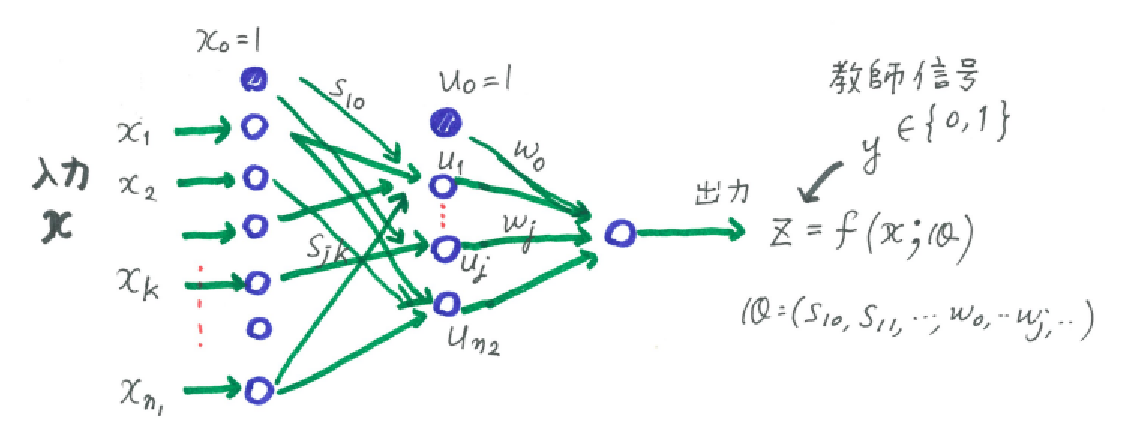
\includegraphics[width=.8\linewidth]{figs/nn20180425.eps}
\caption{3層神経回路モデル(実質は2層)\label{fig:3layer}}
\end{center}
\end{figure}
\end{center}


ニューラルネットには,
いくつかの典型的な要素モデルがある.% \cite{amari88c}.
その一つが,パーセプトロンを代表とする教師あり学習である.
これは,入力とそれに対する望ましい出力のペアが多数与えられることから,
「例からの学習」
\cite{rumelhart86b}
とよばれている.
Deep Learning の問題設定もこれにあたると考えてよい.
\vskip 2mm

ニューラルネットについては,
次のようなイメージを持っておけばよいだろう.
\begin{enumerate}
\item 活動のダイナミクス.
これは「思考」に対応.
個々の素子(ニューロン)は,
他の素子の活動を重み付きの和で受け取り,
自分が興奮するか否かを決定する.

\item 結合のダイナミクス.
これは「学習」に対応.
      「重み」(結合荷重,結合係数)は,
活動のダイナミクスとは比較にならないくらい,
ゆっくり変化する.
学習のダイナミクスとも言う.
学習がローカル(局所的)とは,
$j$番目から$i$番目の素子への
結合荷重$w_{ij}$の変化分が,
$j$番目の素子の活動と$i$番目の素子の活動にのみ依存する学習法則のこと.
誤差逆伝搬法は,ローカルな学習とは考えられていないが,
「活動」をそれぞれの素子がなんらかの形で持っている「信号」と思えば,
      誤差逆伝搬法\cite{rumelhart86b,amari88c,sgeman92a}もローカルな
      学習と解釈できる.

\item 
単純な Yes,No の意思決定をする素子(人間)が多数存在する回路(世界・社会).
本来は,大量の素子が並列に動作する.
結合係数(人と人との信頼関係)は時々刻々ゆっくり変化して形成される,

\end{enumerate}


\section{例からの学習(教師あり学習,パーセプトロンなど)\cite{rumelhart86b,amari88c,sgeman92a}}
%      
\begin{itembox}[l]{問題設定}
      いま入力とそれに対する望ましい出力(教師信号)のペア
      $
      (\bx^1, \by^1),
      (\bx^2, \by^2), \dots
      (\bx^m, \by^m)$ が $m$個,与えられている.
各入出力ペア $(\bx^\alpha, \by^\alpha), \alpha=1,\cdots,m$は,ある未知の確率分布$\Pr(\bx,\by)$にしたがっているとする.
      目的は,$\bx^\alpha$ を入力すると,
      $\by^\alpha$を出力するような
      回路(ネットワーク)$f(\bx;\btheta)$を作ることである.
      ただし,与えられた例題に対してだけではなく,
      未知の入力$\bx$に対しても,
      正しい答え$\by$を出力できる回路を作ることである.


\begin{itemize}
\item given $ \{ (\bx^\alpha, \by^\alpha) \}, \alpha=1,\cdots,m $
 \item find
       $ \btheta^* = {\displaystyle \mathop{\rm argmin}_{\btheta}
       {\rm E} \Bigl [   \frac{1}{2} \Bigl ( f(\bx^\alpha;\btheta) -
       \by^\alpha \Bigr )^2  \Bigr ] }  $
\end{itemize}
\end{itembox}

回路の性質は結合係数の値で決まる.
すべての結合係数をまとめてパラメータ$\btheta=(w_{12},w_{13},\cdots)$で表そう.
回路を設計することは,
関数$f(\bx;\btheta)$を設計することとも言える.
したがって
回路$\approx$関数である.
学習とは,初期値として与えられた不完全なパラメータ$\btheta$の値を,
例題(訓練データ,training set)
${\cal D} = \{
      (\bx^1, \by^1), \dots
      (\bx^m, \by^m)
      \}
      $に合うように変えていくことである.
学習は,パラメータ推定ともいう.
パラメータ$\btheta$は,
例題${\cal D}$に依存して決まるので,
回路$f(\bx;\btheta)$のことを $f(\bx;{\cal D})$とも記述する.


最近出版された機械学習の書籍では,
Tensorflow, Chainer など機械学習のフレームワークを使い,
コンピュータシミュレーションをする方法が
記述されている.
そこを入口にしても悪くはないが,
まず小さい問題を解く回路のコンピュータプログラムをゼロから
書いてみよう.
大規模な回路がどのように動いているか,
動作原理の理解が深まるはずである.


\subsection{課題}
「系統的に」解析する,とはどういうことか知ることを目的にするため,
課題は,
有名な論文\cite{rumelhart86b,sgeman92a}に掲載されている結果を
再現し,その結果を『考察』することとする.
本質的でない点まで再現する必要はない.
どの課題も出力層は1個の出力素子から構成される.
入力層の素子数$n_1$や,
中間層(第2層,隠れ層)の素子数$n_2$は,
課題により異なる.
\rhead{}
\begin{enumerate}
\item XOR ゲートの実現 (入力2次元,$n_1=2, n_2=2,3,\cdots$)
\item mirror symmetry の検出($n_1=6$. \cite{rumelhart86b}の Fig. 1)
 \begin{itemize}
  \item 論文通りの結果が得られない可能性が高い.それはどこに原因があるか.
	隠れ層の素子数 2 でできるのか.考察する価値あり.
  \item 結合係数の初期値,バッチ学習か逐次学習か.

 \end{itemize}



 \item サインカーブで区切られた領域の分類(\cite{sgeman92a}のFig.3)

\begin{enumerate}
 \item nearest-neighbor (\cite{sgeman92a}の
       Fig.4 〜 Fig.7)
 \item feedforward neural network
       ($n_1=2$.\cite{sgeman92a}の
       Fig.8 〜 Fig.11)
\end{enumerate}

\end{enumerate}





\subsection{教師あり学習の原理}
以下,図1に記述した記号を用いて説明する.
入力層に信号$\bx$が与えられると,
第2層の$j$番目の出力 $u_j$が
\begin{eqnarray}
u_j & = & g \left ( \sum_{k=1}^{n_1} s_{jk}x_k - \theta_j \right )
\end{eqnarray}
と計算できる
($j=1,\cdots,n_2$).
ここで,
$s_{jk}$は,第1層$k$番目の素子から第2層$j$番目の素子への
結合の重み,
$\theta_j$は第2層$j$番目の素子のしきい値である.
$g(u)$は,ニューロンの出力関数で
\begin{eqnarray}
g(u) & = & \frac{1}{1 + \text{e}^{-u} } 
\end{eqnarray}
の場合を考える.
ここで $x_0=1$という常に興奮する素子を考えると
\begin{eqnarray}
u_j & = & g \left ( \sum_{k=0}^{n_1} s_{jk}x_k \right )
\end{eqnarray}
と簡潔に記述できる.
$s_{j0} = -\theta_j$のことを素子のバイアスとよぶ.
%
第2層の各素子の出力が決まると,
出力層の素子の出力が
\begin{eqnarray}
 z & = & g \left ( \sum_{j=0}^{n_2} w_j u_j \right ) \\
 & = & g \left ( \sum_{j=0}^{n_2} w_j g \left ( \sum_{k=0}^{n_1} s_{jk}x_k \right ) \right ) 
 \end{eqnarray}
と計算できる($w_0$はバイアス項).
ここで,
$w_j$は,第2層$j$番目の素子から出力層の素子への
結合の重みである.


例題(訓練データ,training set)
${\cal D} = \{
      (\bx^1, y^1), \dots
      (\bx^m, y^m)
      \}
      $が$m$個,与えられているとする.
      入力$\bx^\alpha$に対する望ましい出力が
      $y^\alpha \in \{0,1\}$である
      (現実には $ \lim_{u \rightarrow \infty} g(u)= 1$ なので,
      $y^\alpha \in \{0.1,0.9\}$としたほうがいいかもしれない).
%      $y^\alpha(\bx^\alpha)$と書こう.
いま,目的は,ある入力$\bx$が与えられた時,
\begin{eqnarray}
E & = & \frac{1}{2} 
\sum_{\alpha=1}^{m} 
\left ( z(\bx^\alpha) - y^\alpha \right )^2
\end{eqnarray}
を最小化することだと考えよう,
$E$を損失関数という.
もちろん別の損失関数を定義し,それを最小化してもよい.



パラメータ
$\{s_{jk} \}, \{w_j\}$ は,
初期値として,でたらめな値が設定されている.
したがって,
たとえば信号 $\bx^5$ を回路に入力しても,
出力 $z=z(\bx^5)$ として $y^5$ と同じ値が出力されることは,まずない.
回路が望ましい出力により近い値を出すように,
各パラメータを,
少し大きくするか,小さくするか,変えればよい.
どちらに動かせばよいかは,
$ \frac{\partial E}{\partial w_{j}} $ を計算してみるとよい.
$ \frac{\partial E}{\partial w_{j}} $ が
正の値の場合,
$w_j$ を大きくするると,損失 $E$が大きくなる.
$E$は小さくしたいので,
\begin{eqnarray}
w_j & := & w_j  + \Delta w_{j} =  w_j - \mu \frac{\partial E}{\partial w_{ij}} 
\end{eqnarray}
と更新すればよいだろう
(大きくするか小さくするかが問題で,
動かす大きさを $ \frac{\partial E}{\partial w_{j}} $
に比例させるのがいいか,ということは議論の余地がある).
ここで,
$\mu$は$\mu = 0.05$などの,小さい正の値で,
学習係数とよばれている.
同様に,
$ \frac{\partial E}{\partial w_{j}} $ が
負の値の場合,
$w_j$ を大きくすると$E$が小さくなることを意味している.
損失 $E$は小さくしたいので
やはり
\begin{eqnarray}
w_j & := &  w_j - \mu \frac{\partial E}{\partial w_{ij}} 
\end{eqnarray}
と,更新すれば,損失 $E$は小さくなる.
具体的に,偏微分の項を計算しよう.
%
\begin{eqnarray}
E & = & \frac{1}{2} 
\sum_{\alpha=1}^{m} 
\left ( z(\bx^\alpha) - y^\alpha \right )^2\\
 z & = & g \left ( \sum_{j=0}^{n_2} w_j u_j(\bx^\alpha)\right ) 
 \end{eqnarray}
 であるので,
\begin{eqnarray}
\Delta w_{j} & = & - \mu \frac{\partial E}{\partial w_{j}} 
 = 
-\frac{\mu}{m}
\sum_{\alpha=1}^{m}
\biggl \{
\biggl ( z(\bx^\alpha) - y^\alpha
\biggr )
g' \biggl ( \sum_{j=0}^{n_2} w_j u_j(\bx^\alpha)  \biggr )   u_j(\bx^\alpha) 
\biggr \}
\end{eqnarray}
と書ける.
実は,この更新式を
\begin{eqnarray}
\Delta w_{j}  & = & \mu   r u_j 
\end{eqnarray}
と,
すっきりと解釈する見方がある.
ここで$r$は出力素子が持っているなにかである(あとで学習信号とよぶ).
この更新式は
出力層の素子と中間層の
$j$番目の素子との結合を,$r$との掛け算に比例して更新,という形になっている.
こういう形をHebb 学習という.
信号 $\bx^5$ が回路に入力された場合で学習信号$r$を具体的に考えよう.
\begin{enumerate}
 \item 信号 $\bx^5$ を回路に入力
\item 出力層の素子の内部状態 $ v(\bx^5) = \sum_{j=0}^{n_2} w_j u_j(\bx^5)
      $ を計算.
 \item 出力 $z=g(v(\bx^5))$と望ましい出力との誤差 $ d = z(\bx^\alpha) - y^\alpha $ を計算.
 \item  $ r = -d g'(v(\bx^5)) $ と定義すると(これは出力素子の学習信号),
	入力$\bx^5$に対してだけの変化分は $ \Delta w_{j} = \mu r u_j(\bx^5) $
	と書ける.
$g'(v)$ は素子の出力関数$g(v)$の微分で,
\begin{eqnarray}
g(v) & = & \frac{1}{1 + \text{e}^{-v/T} } 
\end{eqnarray}
の場合($T$はパラメータ)
\begin{eqnarray}
g'(v) & = & \frac{1}{T} g(v) ( 1 - g(v) )
\end{eqnarray}
であり(実際に微分し確認してみよ),
$T=1$の場合,
出力値 $z=g(v) $ であるので,
$ g' = z(1-z) $
と簡単に計算できる.
したがって
\begin{eqnarray}
 r & = &  - (z-y) z (1-z) =  (y -z) z (1-z)
\end{eqnarray}
が学習信号である.
\end{enumerate}

\noindent
{\gt 考察:}
この学習信号の式は面白いので,少しの間,にらめっこして式の意味を考えてみよう.
自分が出力素子(ボス)になった気分になればよくわかる.
$ \Delta w_{j}  =  \mu   r u_j $ であるので,
$r$の正負が重要になる.
$z(1-z)$の項は常に正(もしくは$0$)なので,
とりあえずは気にしないでよいだろう.
いま回路に入力が与えられ,順に計算し,出力を計算(ボスが意思決定)したとする.
回路の出力$z$と望ましい出力$y$が一致している場合,
$r=0$となる.
更新式は,
結合係数の値は更新しなくて良い,ということを意味している.
一方 $y=1$を出力すべきなのに$z=0$だった場合は,
$ \Delta w_{j}  =  \mu   r u_j $ であるので,
出力が正の素子(部下)とは結合を強め(もっと君の意見を尊重すべきだった),
出力が負の素子とは(おまえのせいで間違えた!,ということで)結合を弱めることになる.
逆に,$y=0$を出力すべきなのに$z=1$を出力してしまった場合は,
出力が正の素子とは結合弱め(おまえのせいで間違えた!),
出力が負の素子とは結合を強めることになる.
$r$がの正(負)であるということは,いまよりも,もっと正(負)の値を出力
せよ,という教師信号であると思ってよい.

ここまで出力素子が $0,1$の間の値をとる場合を考えてきたが,
$-1,1$の間をとるモデル
\begin{eqnarray}
 g(v) & = & \tanh(v) = \frac{e^v - e^{-v}}{e^v + e^{-v}}
\end{eqnarray}
を考える場合もよくある\cite{sgeman92a}.
ここで整理しておこう.これを微分すると
\begin{eqnarray}
 g'(v) & = & (1-g(v)^2) = (1-z^2)
\end{eqnarray}
と簡単に書ける(やはり実際に微分し確認しておくこと).
$\{0,1\}$モデルの場合 $z(1-z)$ であった項が,
$(1-z^2)$となるが,
この項も常に$0$以上$1$以下の値をとる(負にはならない)
ことは同じである.
\vskip 5mm


\noindent
{\gt 演習課題:}
$\Delta s_{jk}$ については,自分で計算してみよ
($s_{jk}$が関係している項に○をつけると計算しやすい).\\
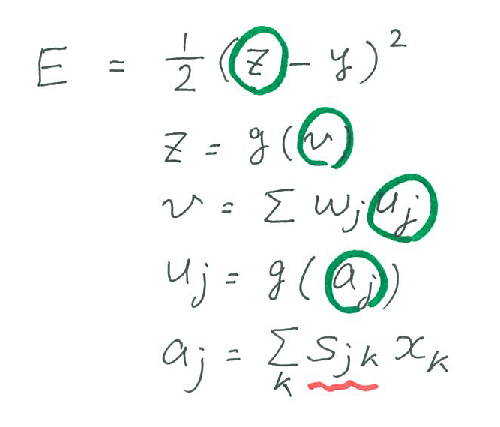
\includegraphics[width=.3\linewidth]{figs/backpropagation_partial_derivative101.eps}
$
\frac{\partial E}{\partial s_{jk}} =
\frac{\partial E}{\partial z} \cdot
\frac{\partial z}{\partial v} \cdot
\frac{\partial v}{\partial u_j} \cdot
\frac{\partial u_j}{\partial a_j} \cdot
\frac{\partial a_j}{\partial s_{jk}} 
$
\vspace*{10mm}

出力層の素子が複数個になった場合について,
バックプロパゲーションの学習式を書いておこう.
Hebb学習を一般化したものであると考えれば,わかりやすい
(図\ref{fig:ghebb}).
\begin{figure}[hbt]
\begin{center}
 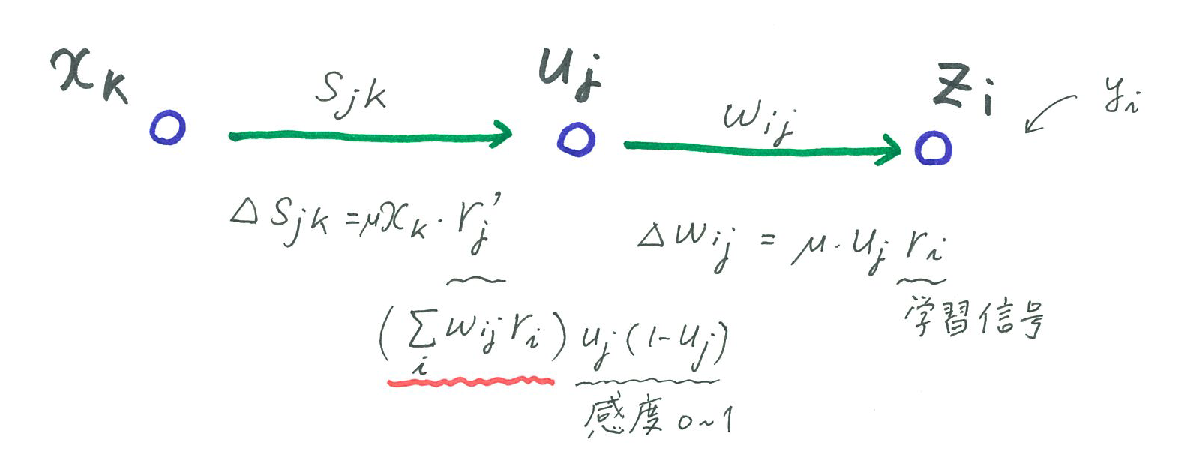
\includegraphics[width=.7\linewidth]{figs/generalized_hebb101.eps}
\caption{入力側の素子の出力と出力側の素子の学習信号とのHebb学習\label{fig:ghebb}}
\end{center}
\end{figure}

第2層の$j$番目の素子と,第3層の$i$番目の素子間の結合の学習は
\begin{eqnarray}
\Delta w_{ij} 
& = & - \mu \frac{\partial E}{\partial w_{ij}} 
 =  -\mu
 \biggl ( z_i(\bx) - y_i(\bx)
\biggr )
g' \biggl ( \sum_{j=0}^{n_2} w_{ij} u_j(\bx)  \biggr )
u_j(\bx) \\
%
& = & -\mu
( z_i - y_i  )
 z_i (1-z_i)
u_j 
\\
& = & \mu r_i  u_j
\end{eqnarray}
と書けるので,
これは第3層$i$番目の素子の学習信号$r_i$と
第2層$j$番目の素子の出力との Hebb学習である
($i=1,\cdots,n_3, j=0,\cdots,n_2$).
第1層$k$番目の素子と第2層$j$番目の素子の結合係数を
$s_{jk}$とすると
\begin{eqnarray}
\Delta s_{jk} 
& = & - \mu \frac{\partial E}{\partial s_{jk}} 
 =  \mu
\left ( \sum_{i=1}^{n_3} w_{ij} r_i \right ) 
g'\left ( \sum_{k=0}^{n_1} s_{jk} x_k \right ) x_k \\
& = & \mu
\left ( \sum_{i=1}^{n_3} w_{ij} r_i \right ) 
u_j(1-u_j)
x_k \\
& = & 
\mu r'_j  x_k
\end{eqnarray}
と,やはり Hebb学習の形で記述できる($k=0,\cdots,n_1, j=1,\cdots,n_2$).
中間層の$j$番目の素子の学習信号$r_j'$が,
出力層の学習信号$r_i$の重み付けの和$ \sum_{i=1}^{n_3} w_{ij} r_i $で計算できる点が,
バックプロパゲーションという名前の由来である.

ここまで3層からなる回路について説明してきたが,層を積み重ねた
100層回路の場合も,
この学習の仕方は変わらない.


ここまで,損失関数
\begin{eqnarray}
E & = & \frac{1}{2} 
\sum_{\alpha=1}^{m} 
\left ( z(\bx^\alpha) - y^\alpha \right )^2
\end{eqnarray}
を最小化することを考えてきた.
ここで,別の損失関数$E$を考えてみる.
最終層の素子の
出力 $ z = f(\btheta | \bx)$ の値は
$0$から$1$の値をとる.
この値を用いると,
「入力$\bx$が与えられたときに,回路が正解を出力する条件付き確率」
は
$ z^y (1-z)^{1-y}$
 と書ける.
 したがって,
 学習を尤度
\begin{eqnarray}
 L & = &
\prod_{\alpha=1}^{m} 
z(\bx^\alpha)^{y^\alpha} (1-z(\bx^\alpha))^{1-{y^{\alpha}}}
\end{eqnarray}
を最大化にするパラメータを求める問題としても定式化できる.
先の2乗誤差最小化の学習と比較するため,
最大化ではなく最小化として定式化すると
\begin{eqnarray}
 E & = &
- \sum_{\alpha=1}^{m} 
\biggl \{ y^\alpha \log z(\bx^\alpha) + (1-y^\alpha) \log \bigl ( 1-z(\bx^\alpha)
       \bigr )  \biggr \}
\end{eqnarray}
となる(対数関数は単調増加関数なので,対数をとっても最小
化すること自体は変わらない).
       これを各結合係数で偏微分した値を計算し,
       2乗誤差誤差最小の場合と結果を比較してみよう.
       例題のインデックス $\alpha$は,手計算に余計なので,記述を省略し
\begin{eqnarray}
 E & = & - \biggl \{ 
    y \log z + (1-y) \log ( 1-z)
\biggl \}
\end{eqnarray}
の偏微分を考えよう(各自,一度手を動かして計算すること).
\begin{eqnarray}
\Delta w_{j} 
& = & - \mu \frac{\partial E}{\partial w_{j}} 
 =  \mu
 \biggl \{
y \frac{1}{z} z(1-z) u_j
+ (1-y)
(-1) \frac{1}{1-z} z(1-z) u_j
\biggl \} \\
 & = &
 \mu
 \biggl \{
y (1-z) u_j
- (1-y)
 z u_j
\biggl \} 
=  \mu
 \biggl \{
y (1-z) 
- (1-y)
 z 
\biggl \} u_j
\\
 & = &
 \mu
(y-z) 
u_j = 
 \mu
 r
u_j
\end{eqnarray}
と,2乗誤差最小の場合と比べ,最終層の素子の学習信号$r$に
感度項 $ z(1-z)$がなくなったものになっている.
このように簡潔に書けるのは,
出力関数として
シグモイド関数 $ g(u)= 1/(1+\exp(-u))$ を用いたおかげである.
この$E$は,
交差エントロピー誤差関数とよばれている.
昔(25年前のニューロブーム)のときは,
そういう言葉はなかった.
単なる尤度最大化である.

%交差エントロピーという言葉は怪しい.
%ちょっと意味を考えてみよう.
%エントロピーとは,
%離散的な変数の場合,$\sum y_i =1$の
%確率分布では
%\begin{eqnarray}
% H & = & - \sum_{i} y_i \log y_i
%  \end{eqnarray}
%  である.
  
\section{補遺(ほい)}
\begin{enumerate}
 \item 学習誤差,汎化誤差
       
      与えられた例題に対して,回路の出力と望ましい出力の
      誤差を学習誤差とよぶ.
      例題だけを丸暗記していれば,これはゼロとすることができる.
      目的は,いまだ経験していない例題に対して,正しい答えを推論することである.
      未知の入力(学習に用いていないデータ)に対しての,
      回路の出力と望ましい出力の
      誤差を汎化誤差(generalization error)とよぶ.
      つまり目的は汎化誤差をゼロにすることである.
      しかも,少ない数の例題が与えられただけで,本質を見抜く力を身につけることが
      できる知性・知能のある機械を作りたい.

 \item Bias/Variance ジレンマ

       これが本課題のメインテーマ.
       二乗誤差は,Bias項と 
       Variance項に分解できる(文献\cite{sgeman92a} p.10).
       $k-$NN やニューラルネットの実験で
       確かめ,考察する.
       
 \item 回帰(regression)

       これは $ {\rm E }  [y | \bx]   $ のこと.
       二乗誤差を最小にするという意味では,これよりよい推定量はない
       (証明は文献\cite{sgeman92a} p.4).
       もちろん,データからは $ {\rm E }  [y | \bx]   $ を推定することは
       できるが,
       本当のところは神様しかわからない.
       
 \item Nearest-Neighbor Regression

       $k-$Nearest-Neighbor とよばれる.
       $k$ には $1$ とか,$5$ などの整数が入る.
       この方法は単純で,分かりやすい.
       まず例題を全部記憶しておく.
       未知の例題 $\bx$が与えられたときには,与えられている例題の中に含まれている,
       $\bx$に近いものから順に$k$個の例題を取り出し推論に使う.
       それらの例題の望ましい出力の$k$個の平均を,推定値として用いればよ
       い.
       極端な場合を考えれば分かりやすい.
       $k=1$ では,入力にもっとも近い例題と同じ出力を,
       $k$が全例題数であれば,全例題の望ましい出力の平均,つまり,どんな
       入力が与えられても同じ出力を,推定値として用いる.
              
 \item Parzen-Window Regression

       例題にガウス分布のような重みを付けて考える.考え方は $k-$NN と同
       じ(といえば,語弊があるかもしれない).

 \item 具体的な実験の仕方(評価の方法)

       ここでは,
       $ {\rm E }  [y | \bx]   $ がわかっている場合で実験するので,
       学習誤差について,
       横軸に時間$t$,縦軸に誤差$E(t)$をプロットした図で評価すれば良い
       
 \item ニューロンの出力を決める関数について.
       
       $g(u) = 1/\{1+\exp(-u)\}$など(活性
       化関数とよばれたりする)は,$0$ から $1$の値を出力する.
       $-1,1$ の値を出力させたければ,
       $g(u) = \tanh (u) $
       を用いていればよい.
       出力層の素子はともかく,
       中間層の素子には,
       $g(u) = \tanh (u) $
       を用いたほうが,学習が速く進む,ようだ(←理論的根拠を調べる必要
       あり).
       出力値の望ましい信号も $0,1$より,
       $ y = \pm 1 $ のときのほうが学習がうまくいくという話もある.
       どちらの場合も,望ましい出力を $0.1,0.9$ とか,
       $-0.9, 0.9$とすると,
       学習が速く進むはずである.
       $g(u) = 1/\{1+\exp(-u)\}$では,実際には$0,1$を出力できないので,
       結合係数の値が発散していく可能性がある.

 \item ReLU

       最近,よく用いられる
       活性化関数.
       どうしてよく用いられるかは,また別の機会に解説.

 \item 結合係数の初期値について

       初期値が,以前に考えられていたよりも,重要であることがわかってい
       る.
       平均$0$,分散$0.1$の正規分布にしたがう乱数を用いるなど,
       かなり小さい値をもつのがよいようだ.
       あまりに小さすぎると,学習に時間がかかるようではある.
       学習係数との兼ね合いなど,職人芸が必要.
              
 \item  最適化($E$の最小化)の方法

	これも職人芸が必要.
	おおくのフレームワークでは,
	最適化の
	オプション,たとえば adam,を選べばよい.
	フレームワークを使わず,
	自分で,一度書いてみること.
	
\item Tensorflow, Chainer などの利用

\end{enumerate}



\section{具体的な実験の仕方}
\begin{enumerate}
\item 例題データの作成
 \item 結合係数の初期値を適当な乱数に設定
 \item 回路に入力を与え,順に素子の出力を計算し,最終出力を計算.
 \item 結合係数の値を更新
 \item 学習がある程度完了するまで,2. に戻って繰り返す.
       学習が進んでいるかどうかは,$E$の値の時間変化をみるとよい.
       振動している場合,学習係数が大きすぎることに原因があると考えよう.
\end{enumerate}

\rhead{}

% BibTeX を使用する場合 %%%%%%%%%%%%%%%%%%%%%%%%%%%%%%%%%
\bibliography{irl_bibs}


\newpage
%
%
\lhead{2018年4月26日\\ 数理脳科学}
\rhead{学籍番号:{\large \underline{\hspace*{15mm}}
\underline{\hspace*{15mm}}}\vspace*{5mm}\\
\underline{名前:\hspace*{5cm}}~
\underline{得点:\hspace*{2cm}}
}
\vspace*{1mm}

\begin{center}
{\large\bf 小テスト 【バックプロパゲーション】}
\end{center}

\begin{enumerate}

\item 
ニューロンの出力関数が
\begin{eqnarray}
f(u) & = & \frac{1}{1 + \text{e}^{-u/T} } 
\end{eqnarray}
の場合を考える($T$は正の定数).
\begin{eqnarray}
f'(u) & = & \frac{1}{T} f(u) ( 1 - f(u) )
\end{eqnarray}
であることを以下の手順で確かめよ.
      

\begin{enumerate}
\item $ 1 - f(u) $ を求めよ.

\vskip 20mm
      
\item $f'(u)$を求めよ. 微分の公式:$ \left \{ \frac{1}{g(u)} \right \}' = - \frac{g'(u)}{\{g(u)\}^2 }$

\end{enumerate}



      \newpage


\begin{figure}[hbt]
\begin{center}
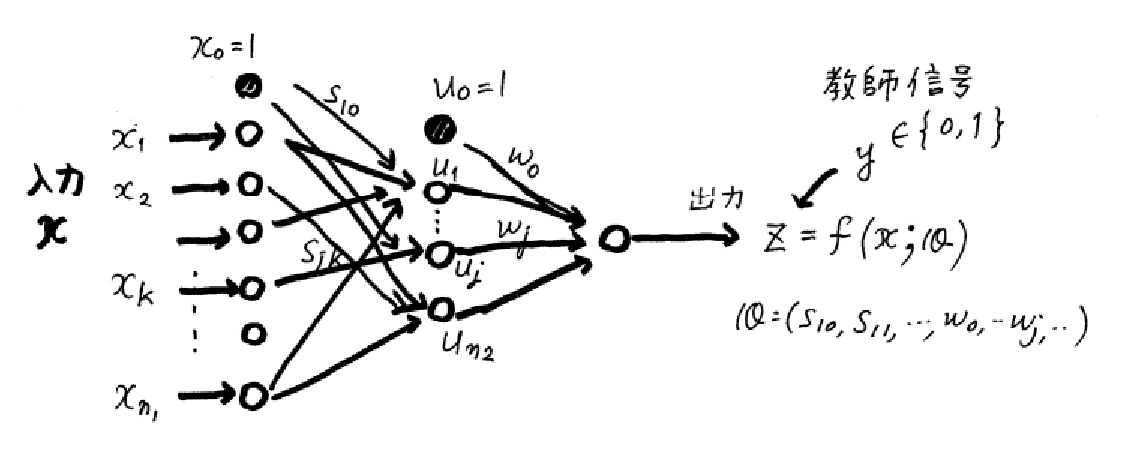
\includegraphics[width=.8\linewidth]{figs/nn20180425bw.eps}
\caption{3層神経回路モデル(実質は2層)\label{fig:3layer}}
\end{center}
\end{figure}


 \item $\bx$が入力されたときの $\Delta s_{jk} = - \mu \frac{\partial
       E}{\partial s_{jk}}
              $ を計算せよ.
$ E =  \frac{1}{2} 
\biggl ( z(\bx) - y \biggr )^2
$
とする.\\
以下,余力がある場合:~
回路の出力 $ z = f(\btheta | \bx)$ を
「入力$\bx$に対し回路が正解を出力する確率」
       と考え,学習の目的を
       尤度 $ z^y (1-z)^{1-y}$
を最大化することと定式化できる.
最小化する関数を
       $ E= - \biggl \{ y \log z(\bx) + (1-y) \log \bigl ( 1-z(\bx)
       \bigr )  \biggr \}$
       (対数尤度の符号を反転したもの)
       と定義した場合についても,各結合係数で偏微分した値を計算し,
       2乗誤差誤差最小の場合と結果を比較してみよ.
       

% \vskip 200mm
       \newpage
       


 \item 
      $ E \biggl [ \biggl ( y-f(\bx; \btheta) \biggr )^2 \bigg | \bx \biggr ] \geqq
E \biggl [ \biggl ( y-E[y | \bx] \biggr )^2 \bigg | \bx \biggr ] 
       $を証明せよ.
\vspace*{2mm}
       
       ここで,$f(\bx)$は回路の出力,
 %      (正確には$f(\bx;{\cal D})$ もしくは $f(\bx;\btheta)$ ),
       $y$は望ましい出力(一次元,$\by=y$),
       $E$は入力$\bx$に対する期待値.
       この不等式の意味:
       パラメータ$\btheta$を調節して,
       どんなによい回路$f(\bx;\btheta)$を作れたとしても,
       $E[y | \bx]$ より
       適切な回路は作れない
       (二乗誤差を最小にするという意味で.
       Among all functions of $\bx$,
       the regression is the {\it best} predictor of $y$
given $\bx$, in the mean-squared-error sense.
       ).
       ※ $E[y|\bx]$は$\bx$の決定的な関数,回帰(regression)という.


\newpage
% \vspace*{20cm}



 \item 
       $ E_{\cal D} \biggl [ \biggl ( f(\bx;{\cal D}) - E[y|\bx] \biggr )^2  \biggr ]
       =
       \biggl ( E_{\cal D} \bigl [ f(\bx;{\cal D}) \bigr ] - E[y|\bx] \biggr )^2
       + E_{\cal D} \biggl [ \biggl ( f(\bx;{\cal D}) - E_{\cal D} \bigl
       [f(\bx;{\cal
       D}) \bigr ] \biggr )^2\biggr ]
$
       を証明せよ.右辺第一項をバイアス項,第二項をバリアンス項という.
$E_{\cal D}$は,訓練データ集合${\cal D}$に関して期待値をとる操作.
       \vspace*{2mm}

\end{enumerate}

\end{document}

